%!TEX root = ../thesis.tex
%*******************************************************************************
%****************************** Fourth Chapter *********************************
%*******************************************************************************
\chapter{Determinants of cross-tissue cell type identity and distribution} \label{chap:CT_bio}

% **************************** Define Graphics Path **************************
\ifpdf
    \graphicspath{{Chapter4/Figs/Raster/}{Chapter4/Figs/PDF/}{Chapter4/Figs/}}
\else
    \graphicspath{{Chapter4/Figs/Vector/}{Chapter4/Figs/}}
\fi
Cell identity can be defined by the genes it expresses. A continuously increasing number of studies has applied scRNA-seq to profile cells from various body locations and describe the cells that make up a tissue, in the steady-state or disease. A smaller number of studies have focused on the differences between the cell types detected in different tissues~\citep{miragaia_single-cell_2019,scott_transcription_2018}. However, we don't yet know how variable transcriptome of most cell types is between tissues, and how it relates to the tissue transcriptome.

This Chapter outlines the construction of a human cell type reference based on single-cell transcriptomics, by applying the \textit{CellTypist} framework presented in Chapter~\ref{chap:CT_method}. The present Chapter will focus on the interpretability of this pipeline, and reveal the genes driving cell identity across tissues. We will further dissect the relationships across tissues established by \textit{CellTypist}, and explore the influence of different major cell types in tissue biology.

The work presented in this Chapter was partly developed with the assistance of Ni Huang, who contributed to the collection and integration of published datasets. The analyses here performed are based on the methodology outlined in Chapter~\ref{chap:CT_method}. Supplementary figures are included in Appendix~\ref{appendix:CTsub}.


\section{Introduction}
\label{section4.1}
% defining and cataloguing cell types
The definition of cell type is, like many in biology, a working concept. Cells have been classified based on different aspects of their morphology, molecular phenotype, or function. Historically, this knowledge of cell identity has been restricted to their fields of study, hindering the development  of an integrative, systemic perspective of cell types in the body. Single-cell RNA-seq technologies (scRNA-seq) are now challenging this perspective, since they allow for an unbiased profiling of cell identity through the transcriptome. As scRNA-seq data acquisition grows~\citep{svensson_exponential_2018}, so does our understanding of the cellular make up of the profiled tissues. The Human Cell Atlas Consortium has defined as one of its goals to develop a cellular taxonomy~\citep{regev_human_2017}, which is necessarily harmonised across tissues. Nonetheless, a unified, transcriptome-driven perspective of cell identity is still lacking.

% understanding tissue and cell function
The molecular basis for the relationships between tissues were initially probed by high-throughput methods; first microarrays~\citep{enard_intra-_2002}, and later with RNA-seq~\citep{mortazavi_mapping_2008,brawand_evolution_2011,barbosa-morais_evolutionary_2012}. More recent studies are now linking this transcriptome cross-tissue  variability with genome variants~\citep{consortium_genotype-tissue_2015,gtex_consortium_genetic_2017}, unravelling the regulatory determinants behind tissue biology. Further analysis have delved into the importance of transcription factors for tissue identity~\citep{sonawane_understanding_2017}, revealing that tissue specificity lies not only in these molecules but mostly on the tissue-specific regulatory roles they play, while also showing that transcription factors are less likely to be identified as tissue-specific than other genes. An integrated predictive model of cell identity should be able to reveal patterns relating tissues through cell identity relationships, as well as offer a broad perspective of the genes determining cell types.

% this chapter
Here we will expand on the \textit{CellTypist} pipeline previously defined, and how it can be used to probe cellular identity in human primary cells across body locations. We detail the collection and integration of various human datasets, totalling close to 1.5 million cells from 21 tissues. After applying \textit{CellTypist}, its integrated results are examined for cross tissue relationships. The pipeline can recapitulate known tissue associations, caused either by comparable cell sampling (e.g. tissues solely profiled for immune cells), or by functional similarity. These are evident both at the tissue integration stage, as well as in the top genes learned by the model that define cell groupings in each tissue. These genes are further examined for patterns in cell identity definition, revealing a global pattern for genes coding for functional effector molecules (i.e. receptors and secreted proteins) to be more pivotal in defining cell identity than others involved in genomic regulation. Finally, we discuss on the potential uses and implementation of a scRNA-seq-derived cell type reference.


\section{Results}
\label{section4.2}
\subsection{Human data collection and organisation}
\label{section4.2_coll}
To obtain a global, cross-tissue perspective of human cell types, we obtained a broad representation of single-cell transcriptomes with by collecting several publicly available scRNA-seq datasets (Table~\ref{table:tab_4_1}). Information about tissue, scRNA-seq protocol, sampling method, and cell type annotation (when available) were obtained from the respective publications and data repositories, together with the gene expression matrices.

% table: Dataset; number of cells; ref
\begin{table}[ht!] % p for putting it in the next page available
\footnotesize
\caption[Datasets collected and references]{Datasets collected and references}
\centering
\label{table:tab_4_1}

\begin{tabular}{l|c|r}
\toprule
~\textbf{Dataset} & ~\textbf{Reference} & ~\textbf{\# cells} \\
\midrule
baron16 & ~\citep{baron_single-cell_2016} & 8.569  \\

bjorklund16 & ~\citep{bjorklund_heterogeneity_2016} & 648  \\

gierahn17 & ~\citep{gierahn_seq-well:_2017} & 3.694  \\

guo18 & ~\citep{guo_adult_2018} & 12.053  \\

habib17 & ~\citep{habib_massively_2017} & 14.963  \\

hcaImmune18 & \href{data.humancellatlas.org}{HCA Data Portal} & 593.844  \\

henry18 & ~\citep{henry_cellular_2018} & 109.061  \\

jaitin19 & ~\citep{jaitin_lipid-associated_2019} & 13.199  \\

james20 & \textit{Unpublished} & 32.228  \\

lamanno16 & ~\citep{la_manno_molecular_2016} & 1.977  \\

li19 & ~\citep{li_memory_2019} & 1.886  \\

masuda19 & ~\citep{masuda_spatial_2019} & 6.144  \\

menon18 & ~\citep{menon_single-cell_2018} & 9.846  \\

miragaia18 & ~\citep{miragaia_single-cell_2019} & 1.168  \\

muraro16 & ~\citep{muraro_single-cell_2016} & 2.126  \\

nowakowski17 & ~\citep{nowakowski_spatiotemporal_2017} & 4.261  \\

popescu19 & ~\citep{popescu_decoding_2019} & 113.063  \\

segal19 & ~\citep{segal_single_2019} & 1.475  \\

segerstolpe16 & ~\citep{segerstolpe_single-cell_2016} & 3.363  \\

smillie19 & ~\citep{smillie_intra-_2019} & 110.110  \\

sohni19 & ~\citep{sohni_neonatal_2019} & 34.729  \\

takeda19 & ~\citep{takeda_single-cell_2019} & 33.257  \\

vento18 & ~\citep{vento-tormo_single-cell_2018} & 69.883  \\

vieira19 & ~\citep{braga_cellular_2019} & 26.013  \\

wang16 & ~\citep{wang_single-cell_2016} & 635  \\

young18 & ~\citep{young_single-cell_2018} & 44.526  \\

zhang18 & ~\citep{zhang_lineage_2018} & 5.989  \\

zheng17 & ~\citep{zheng_massively_2017} & 163.234  \\
\midrule
\textbf{\textit{Total}} &  & 1.421.944  \\

\bottomrule
\end{tabular}
\end{table}

\begin{figure}[ht!]
    \centering    
    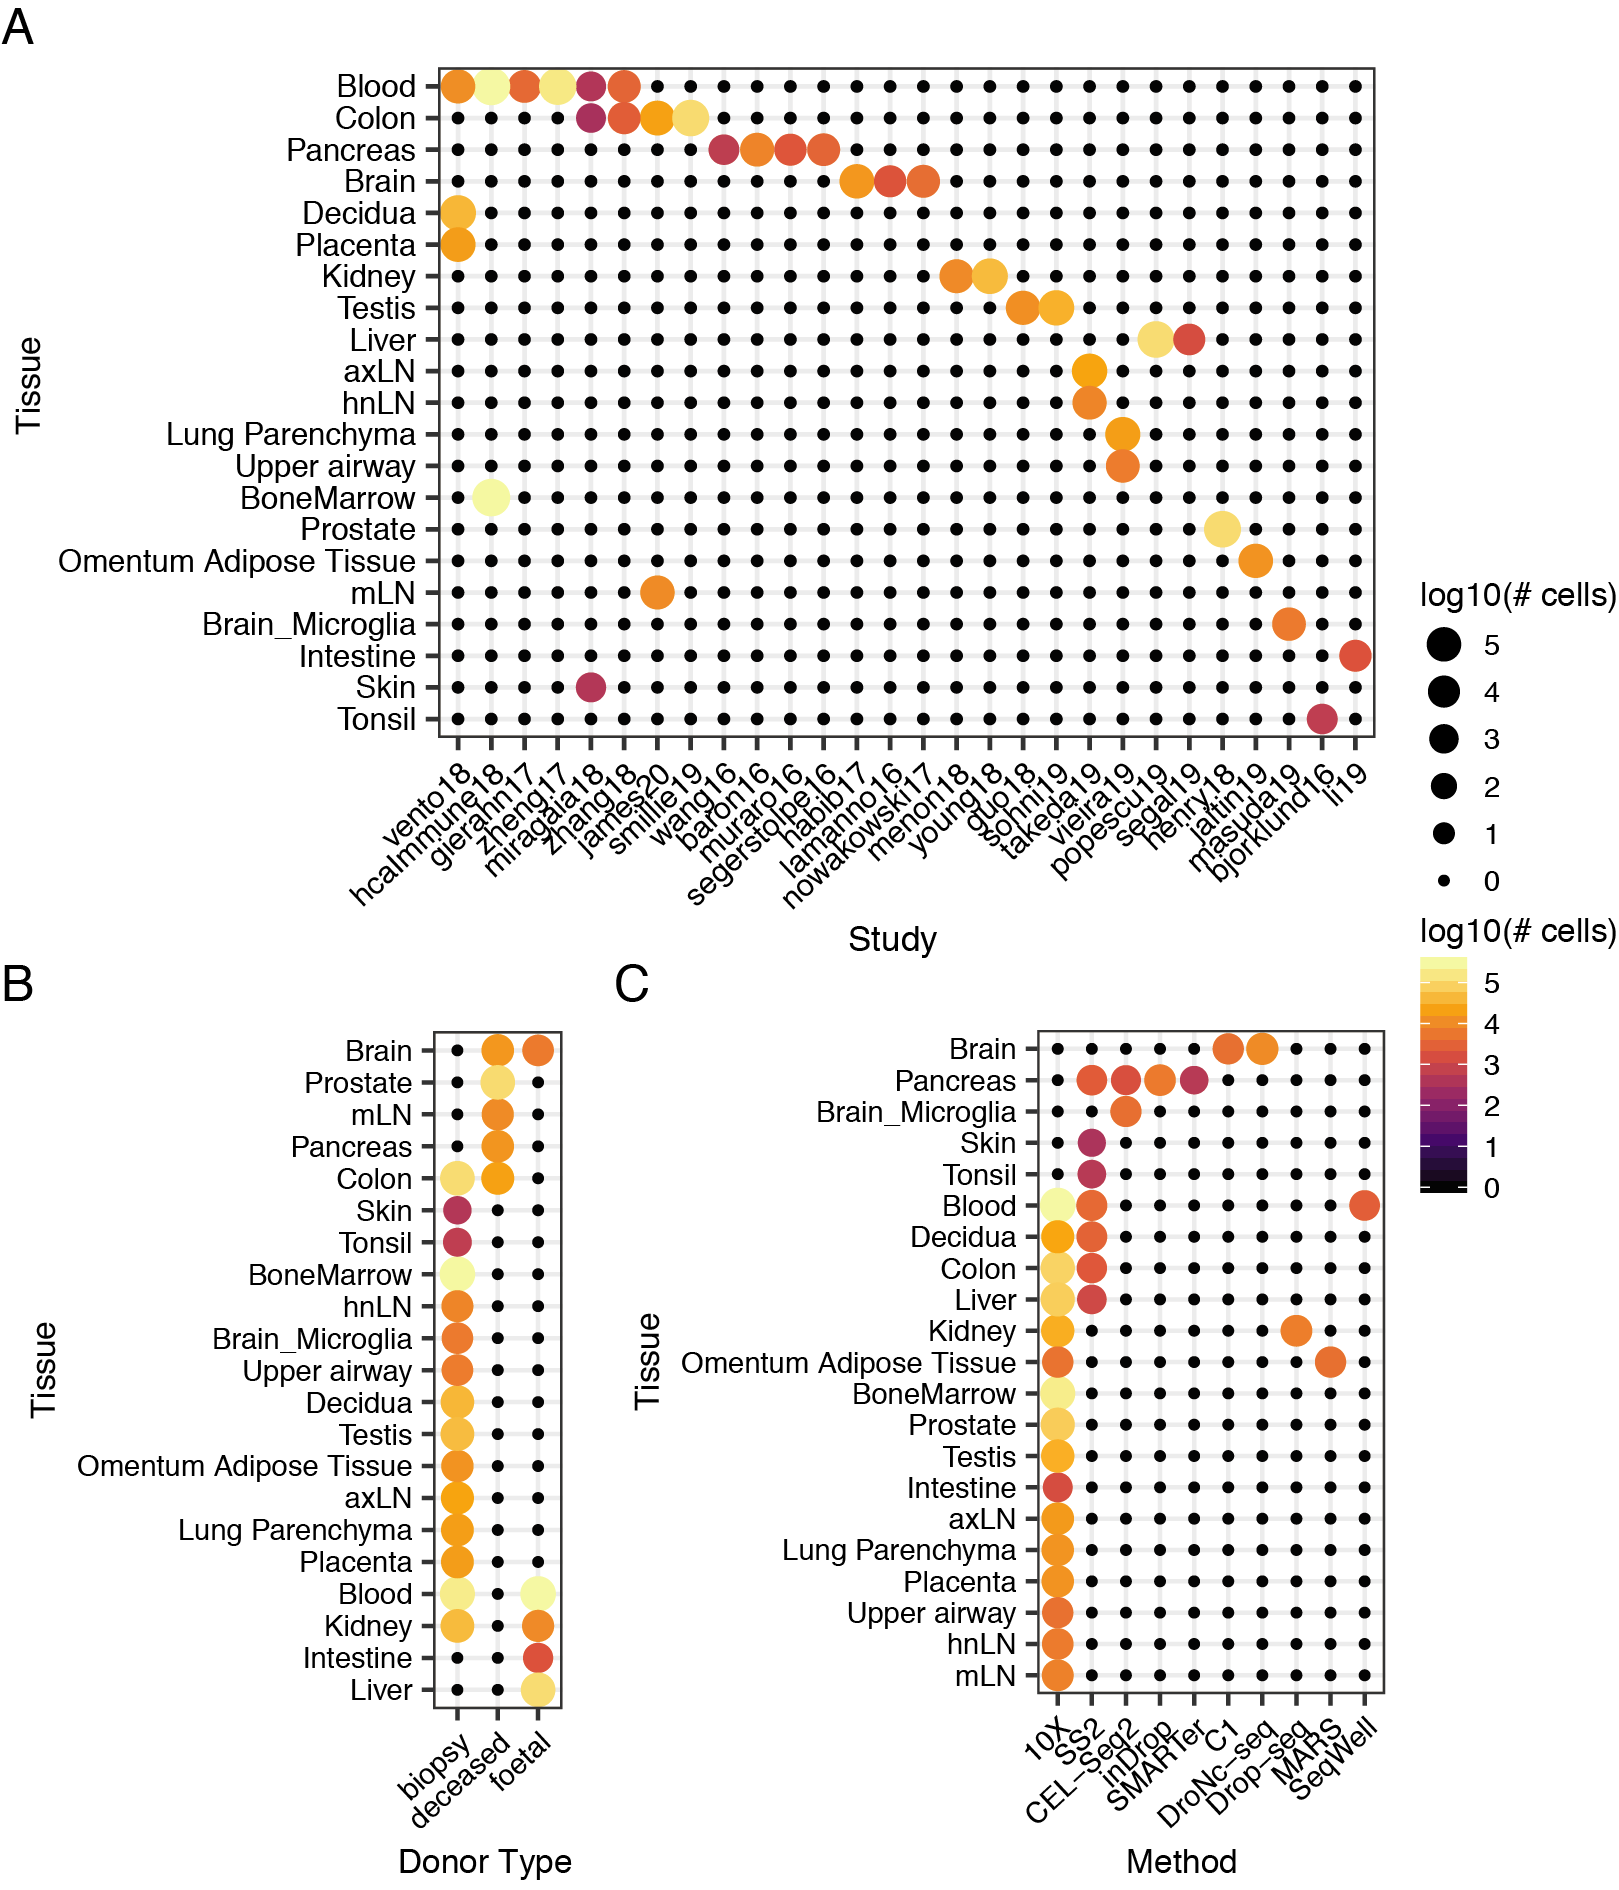
\includegraphics[width=1.0\textwidth]{Chapter4/Figs/chap4_countsHumanAtlas.png} % change word in curlies to change figure
    \caption[Cell numbers in the human dataset collection]{\textbf{Cell numbers in the human dataset collection} \newline Number of cells, in log10 scale, collected from different tissues, and distributed by publication \textbf{(A)}, type of collection \textbf{(B)}, and scRNA-seq protocol \textbf{(C)}.}
    \label{fig:chap4_cha}
\end{figure}

The 28 datasets collected include 21 tissues, mostly collected from adult biopsies (Figure~\ref{fig:chap4_cha}A and ~\ref{fig:chap4_cha}B), and totalling close to 1.5 million cells. Various studies focus on haematopoietic-derived cells, and as such many of the sampled tissues are mostly composed of immune cells (Figure~\ref{fig:appB_ptprc}). Most cells are obtained using the droplet-based "Chromium" instrument from 10x Genomics ("10X" in Figure~\ref{fig:chap4_cha}C), followed by the plate-based, full-length Smart-seq2 ("SS2"). Despite this unbalance in usage of different technologies, it is in agreement with what has been reported in an exhaustive curated reference of single-cell sequencing datasets~\citep{svensson_curated_2019}.

The collected expression matrices for the listed datasets were combined, and gene references were matched across all datasets (Methods Section~\ref{section4.4_datacol}). This was done to maintain the integrity of each dataset, as well as facilitate data collection and incorporation (see Section~\ref{section4.3}). The \textit{CellTypist} pipeline was then applied to this collection (see Methods Section~\ref{section4.4_model}), and parameter optimisation was done as described in the previous chapter, first selecting for each tissue a clustering resolution that yielded the lowest split-join distance between clusters and available cell type annotations (Figure~\ref{fig:chap4_HA}A), and then choosing the set of merged clusters that most resemble the existing cell type annotations in each dataset (Figure~\ref{fig:chap4_HA}B). Applying the optimised parameter combination (thr1 = 0.99, thr2 = 0.8, see Figure~\ref{fig:chap3_combcl}A) resulted in 627 clusters (Figure~\ref{fig:appB_grids}A). An example of a tissue (pancreas) with consistently annotated cell types across datasets can be seen in Figure~\ref{fig:appB_panc}. Using these clusters, a model was then trained as previously shown (Figure~\ref{fig:chap3_model}A, Methods Section~\ref{section4.4_model}) with a classification accuracy of 84\% on left-out test data (Figure~\ref{fig:chap4_HA}C). The F1 statistic calculated for each label was in most cases above 0.75, meaning elevated precision and recall in the model, especially for clusters with more than 100 cells, as previously shown (Figure~\ref{fig:chap3_model}C, Figure~\ref{fig:chap3_modelcl}C).

\begin{figure}[ht!]
    \centering    
    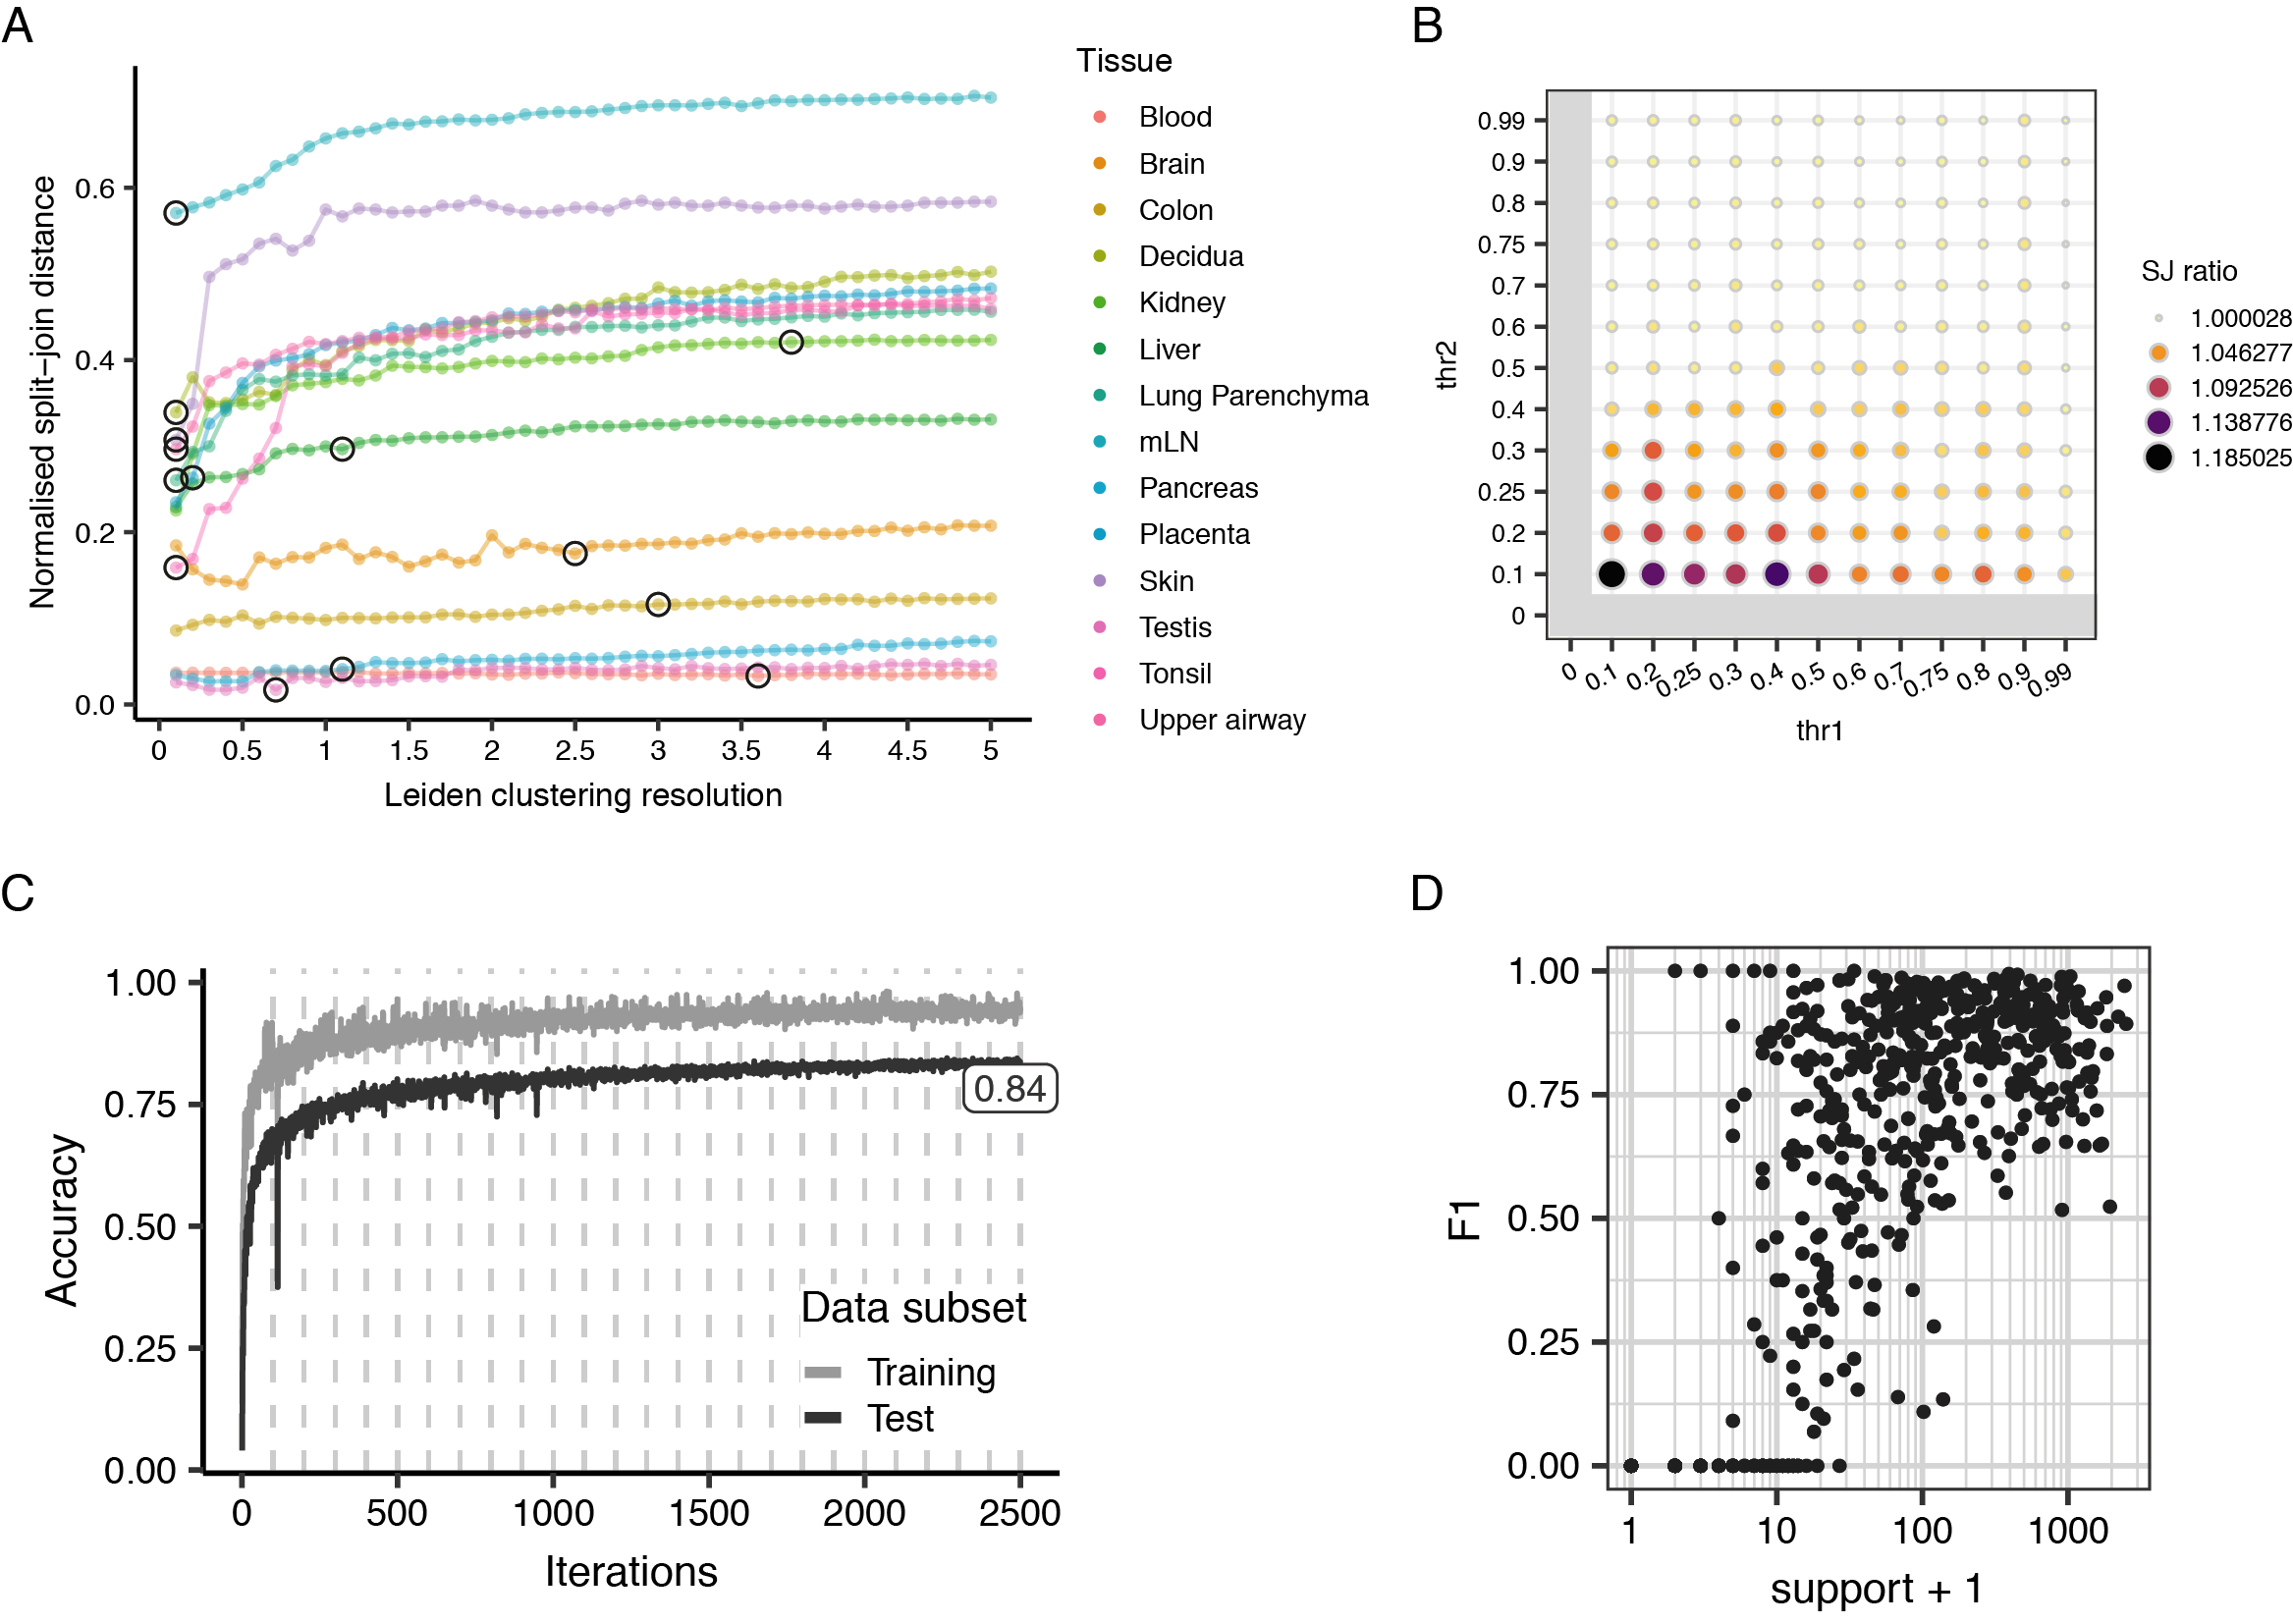
\includegraphics[width=1.0\textwidth]{Chapter4/Figs/chap4_figHA.png} % change word in curlies to change figure
    \caption[Running \textit{CellTypist} on a human scRNA-seq data collection]{\textbf{Running \textit{CellTypist} on a human scRNA-seq data collection}\newline\textbf{(A)} Per-tissue cluster optimisation, choosing the resolution that approximates existing cell type annotations. Similarity is measured with normalised split-join distance, and constrained to solutions with a number of clusters of at least as many as existing annotations in the largest collected dataset. Selected values are indicated with a black circle. \textbf{(B)} Grid of parameters tested for cross-tissue cluster merging, showing the variation of the ratio of split-join distance between merged clusters and cell type annotation, and per-tissue clusters and cell type annotation (colour and size of points). \textbf{(C)} Accuracy during model fitting for training and held-out test data, to predict cross-tissue integrated clusters obtained using thr1 = 0.99 and thr2 = 0.8 as parameters for \textit{CellTypist} (optimal value in (B)). Vertical dashed lines represent each training epoch. Terminal label indicated final accuracy for prediction in the test set. \textbf{(D)} F1-score for each cluster label (black dots) as a function of class size (in log10 scale).}
    \label{fig:chap4_HA}
\end{figure}

Three additional models, trained using sets of clusters derived using different parameters, were also examined. These were thr1 = 0.4 and thr2 = 0.99 (Figure~\ref{fig:appB_moremodels}A-B), thr1 = 0.25 and thr2 = 0.25 (Figure~\ref{fig:appB_moremodels}C-D), and thr1 = 0.1 and thr2 = 0.1 (Figure~\ref{fig:appB_moremodels}E-F, see Methods Section~\ref{section4.4_model}). These models show a lower performance, in particular the latter (thr1 = 0.1 and thr2 = 0.1), with a test classification accuracy of 73\%. This may be due to the excessive merging of clusters within and across tissues, thus leading to hybrid, undetermined groups of cells (Figure~\ref{fig:appB_tissrel}). Other models are more conservative in this regard, and show a better classification performance. The model using clusters obtained with thr1 = 0.25 and thr2 = 0.25 still has noticeably worse values for the split-join distance, yet also represents a more condensed cell type reference (420 clusters), without sacrificing accuracy (83\%). Lastly, the model with the parameters thr1 = 0.4 and thr2 = 0.99, in particular, is the one showing the greatest improvement in matching annotated cell types after cross-tissue merging, and is thus another possible reference model.

In sum, the collected datasets allow for the training of the \textit{CellTypist} pipeline and construct a fully interpretable human cell type reference.


\subsection{Matching cell identity across tissues}
\label{section_tissues}
The clusters detected per tissue using \textit{CellTypist} are independent of the number of datasets (Spearman Rank Correlation = -0.01), although moderately correlated with the number of cells present in each tissue (Spearman Rank Correlation = 0.52) (Figure~\ref{fig:appB_clustnumbs}). The subsequent cluster merging step draws a map of cell identity relationships across tissues. Examining this map can reveal higher order relationships between the tissues present in the global dataset. Thus, the per-tissue classification probabilities used to construct the cluster matching graph (Figure~\ref{fig:chap3_combcl}A) were used to calculate the mean probability of cells from a per-tissue (non-merged) cluster matching the clusters of all tissues. The resulting tissue-by-cluster mean probability matrix is represented in the clustered heatmap of Figure~\ref{fig:chap4_tiss}A. This plot shows that about a third of all clusters have an average high confidence assignment across tissues (bottom of the heatmap), with the remaining two-thirds having much lower per-tissue mean probabilities. Nonetheless, the clustering of these values reveals a stark division between tissues whose immune compartment was predominantly profiled (left major branch of dendrogramme), and those with a more global or non-immune profiling (right branch). This is highlighted by the per tissue mean expression of \textit{PTPRC}, the gene encoding for the CD45 receptor, which is exclusively expressed in immune cells~\citep{altin_role_1997} (Figure~\ref{fig:appB_ptprc}). Expression of \textit{EPCAM} - an epithelial cell marker - and \textit{CD34} - and endothelial cell marker - further illustrate this division, being most expressed in tissues in the opposite dendrogramme branch. We can thus conclude that the cluster matches across tissues are driven by cell identity, in particular by its major lineage (immune, epithelial, endothelial, among others).

\begin{figure}[pht!]
    \centering    
    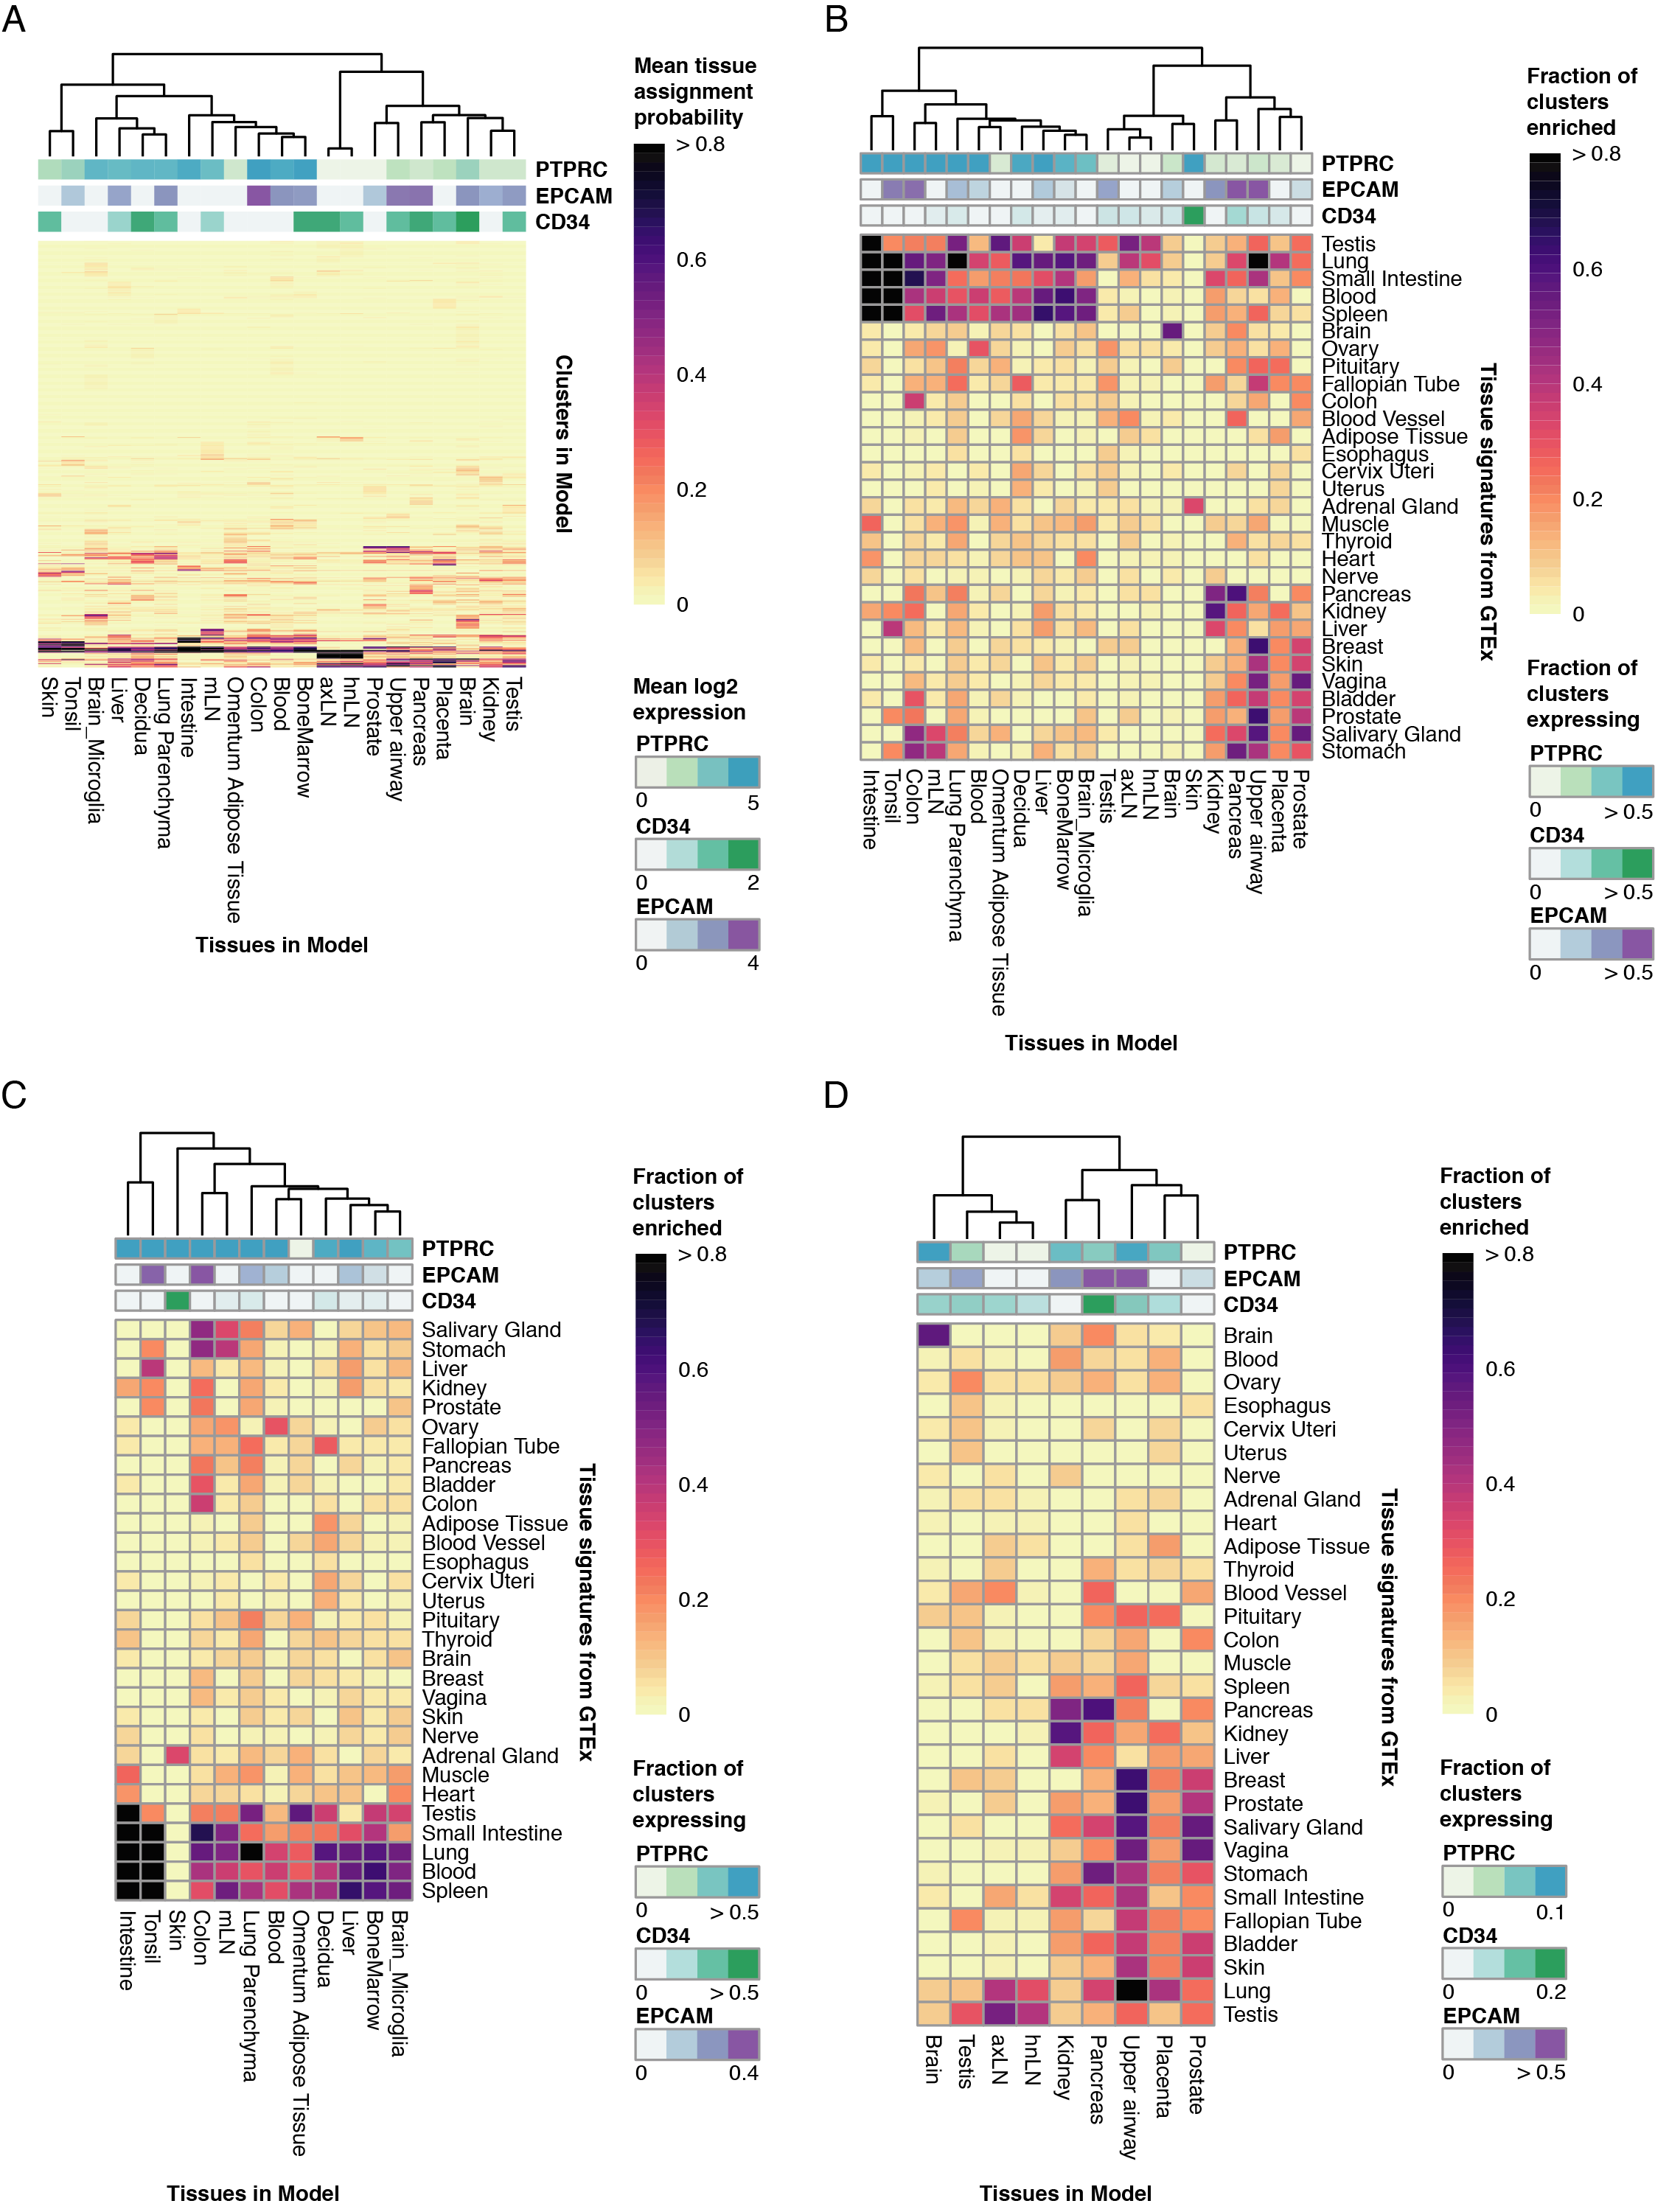
\includegraphics[scale=0.75]{Chapter4/Figs/chap4_tissuefig.png} % change word in curlies to change figure
    \caption[Cell identity relationships across tissues]{\textbf{Cell identity relationships across tissues}\newline\textbf{(A)} Heatmap of the mean assignment probability of cells from a per-tissue cluster to the clusters of each given tissue in the dataset. \textbf{(B)} Heatmap of the fraction of clusters from a given tissue whose \textit{CellTypist} model signature is enriched in certain tissue-specific genes. \textbf{(C and D)} Two major branches of the column dendrogramme in (B), showing the immune enriched (C) and depleted (D) tissues. "Skin" was regrouped due to being an outlier grouped with the non-immune tissues in (B).}
    \label{fig:chap4_tiss}
\end{figure}

Tissue identity is also reflected in gene expression, and therefore in the genes with the top coefficients determined by the \textit{CellTypist} model. To unbiasedly probe the existence of tissue-specific signatures in the top genes of all clusters, tissue signatures were derived from the GTEx Consortium bulk RNA-seq dataset~\citep{consortium_genotype-tissue_2015} (see Methods Section~\ref{section4.4_genelists}). This provided an independent reference for tissue identity using gene expression. Inspection of tissue identity enrichment in cell clusters per tissue (Figure~\ref{fig:chap4_tiss}B) shows that, despite the sets of tissues in the \textit{CellTypist} and GTEx datasets not being completely overlapping, matching between them is mostly concordant. Clustering of the enriched cluster fractions per tissue once again uncovered a similar picture as before, with a clear division between tissues immune enriched and immune depleted tissues. The two cases that seem misaligned from \textit{PTPRC} expression - Omentum Adipose Tissue and Skin - both have an enrichment in immune cells. In the first, low PTPRC fraction is likely derived from general low expression of this receptor. In the case of skin, the misclustering is likely related to the low number of clusters, as well as the specific cell types that make up the sample (Treg and Tmem cells~\citep{miragaia_single-cell_2019}). 

Tissues for which a large number of immune cells were obtained (either by biased sampling or because that is its real nature) had more clusters enriched in signatures of tissues composed of a large number of immune cells ("Blood", "Spleen"), as well as other barrier tissues, which potentially would include greater number or activity of immune cells ("Lung", "Small intestine") (Figure~\ref{fig:chap4_tiss}C). The clustering of the profiled tissues (top dendrogramme of Figure~\ref{fig:chap4_tiss}C) revealed further relationships between them. Tonsil and intestine are grouped together likely due to their sampling bias: ILCs in tonsil, CD4\textsuperscript{+} T memory cells in intestine; and both of these cell types can have globally similar signatures. The clustering of liver and bone marrow is also expected, given that the vast majority of liver samples are from fetal origin, and reflect the organ's haematopoietic function at that stage of development. Lastly, the similarity between colon and the mesenteric lymph node (mLN) point towards a greater similarity between leukocyte populations present in both than with those from other tissues. However, an increase in sampling of immune cells from other lymph nodes and non-lymphoid tissues would further unravel their true relationships.

For the non-immune fraction (Figure~\ref{fig:chap4_tiss}D), cross tissue relationships could also be identified. Axilary (axLN) and head and neck (hnLN) lymph nodes were grouped together since both are uniquely sampled for endothelial cells only, in the same study~\citep{takeda_single-cell_2019}. They are outliers together with testis and brain, two tissues that have been repeatedly described has having very distinct transcriptomic profiles from other organs~\cite{brawand_evolution_2011,barbosa-morais_evolutionary_2012}. The brain clusters very uniquely match the "Brain" gene set, and clusters from testis are in their majority enriched for "Testis" signature as well as "Ovary". The remaining tissues grouped together show elevated enrichment in a group of signatures coming in their majority from barrier tissues ("Lung", "Bladder", "Skin", "Stomach", "Vagina"), as well as some tissues with secretory activity ("Salivary gland", "Prostate", "Breast"). This shows the difference in cellular function of these tissues compared with the immune group, and correlated with the functions of the tissues present (kidney, pancreas, upper airway, placenta and prostate).

The tissue relationships highlighted by the gene set enrichment directly derive from the \textit{CellTypist} model trained and the cell groupings that the pipeline defines. Examining other model alternatives shows that in some of them the tissue hierarchy is maintained (Figure~\ref{fig:appB_tissGSEA}), with the exception of the thr1 = 0.1, thr2 = 0.1 model. This is likely to be caused by excessive merging of clusters, leading to non-meaningful groupings and not so meaningful coefficients from the model.

%paragraph about the matching clusters
Plotting the clusters resulting from cross-tissue merging in \textit{CellTypist} can also reveal the similarity across tissues (Figure~\ref{fig:appB_tissrel}). As already shown by Figure~\ref{fig:appB_grids}, the model with thr1 = 0.99 and thr2 = 0.8 is the one with the lowest number of merged clusters. We can however still observe clusters merging across tissues that have similar profiles and were included in the "immune enriched" group in Figure~\ref{fig:chap4_tiss}B - liver and bone marrow, lung parenchyma and intestine, decidua and omentum adipose tissue - as well as tissues that have functional associations - decidua and placenta, upper airway and lung parenchyma. The remaining models appear to maintain the occurrence of these associations between tissues, like the close clustering between axLN and hnLN, or the association of tissues including more immune sampling with blood and bone marrow. This is further underscored when the tissue gene signatures are examined in the merged clusters of each model (Figure~\ref{fig:appB_clmGSEA}). While the first model (thr1 = 0.99 and thr2 = 0.8) does not include enough merged clusters, both thr1 = 0.4 and thr2 = 0.99 and thr1 = 0.25 and thr2 = 0.25 again present the distinctive pattern of clustering the tissue signatures by the tissue functions as described before for the immune/non-immune partitions. This however is not evident for thr1 = 0.1 and thr2 = 0.1, likely due to excessive merging leading to a less meaningful model.

In conclusion, \textit{CellTypist} can reveal the relationships of cell identity across tissue, and relate it to a more structured hierarchy of cellular phenotypes (such as immune vs non-immune). However, this is also dependent of the profiled tissues, as well as how balanced for all cell populations those samplings are conducted.


\subsection{Gene expression driving cell identity}
\label{section_genes}
Usage of logistic regression as a classification model in \textit{CellTypist} allows for a direct evaluation of the genes driving the classification for each cluster through their learned coefficients. With a comprehensive cell type reference, we can start to unravel what are the key determinants of cell identity across tissues.

\begin{figure}[pht!]
    \centering
    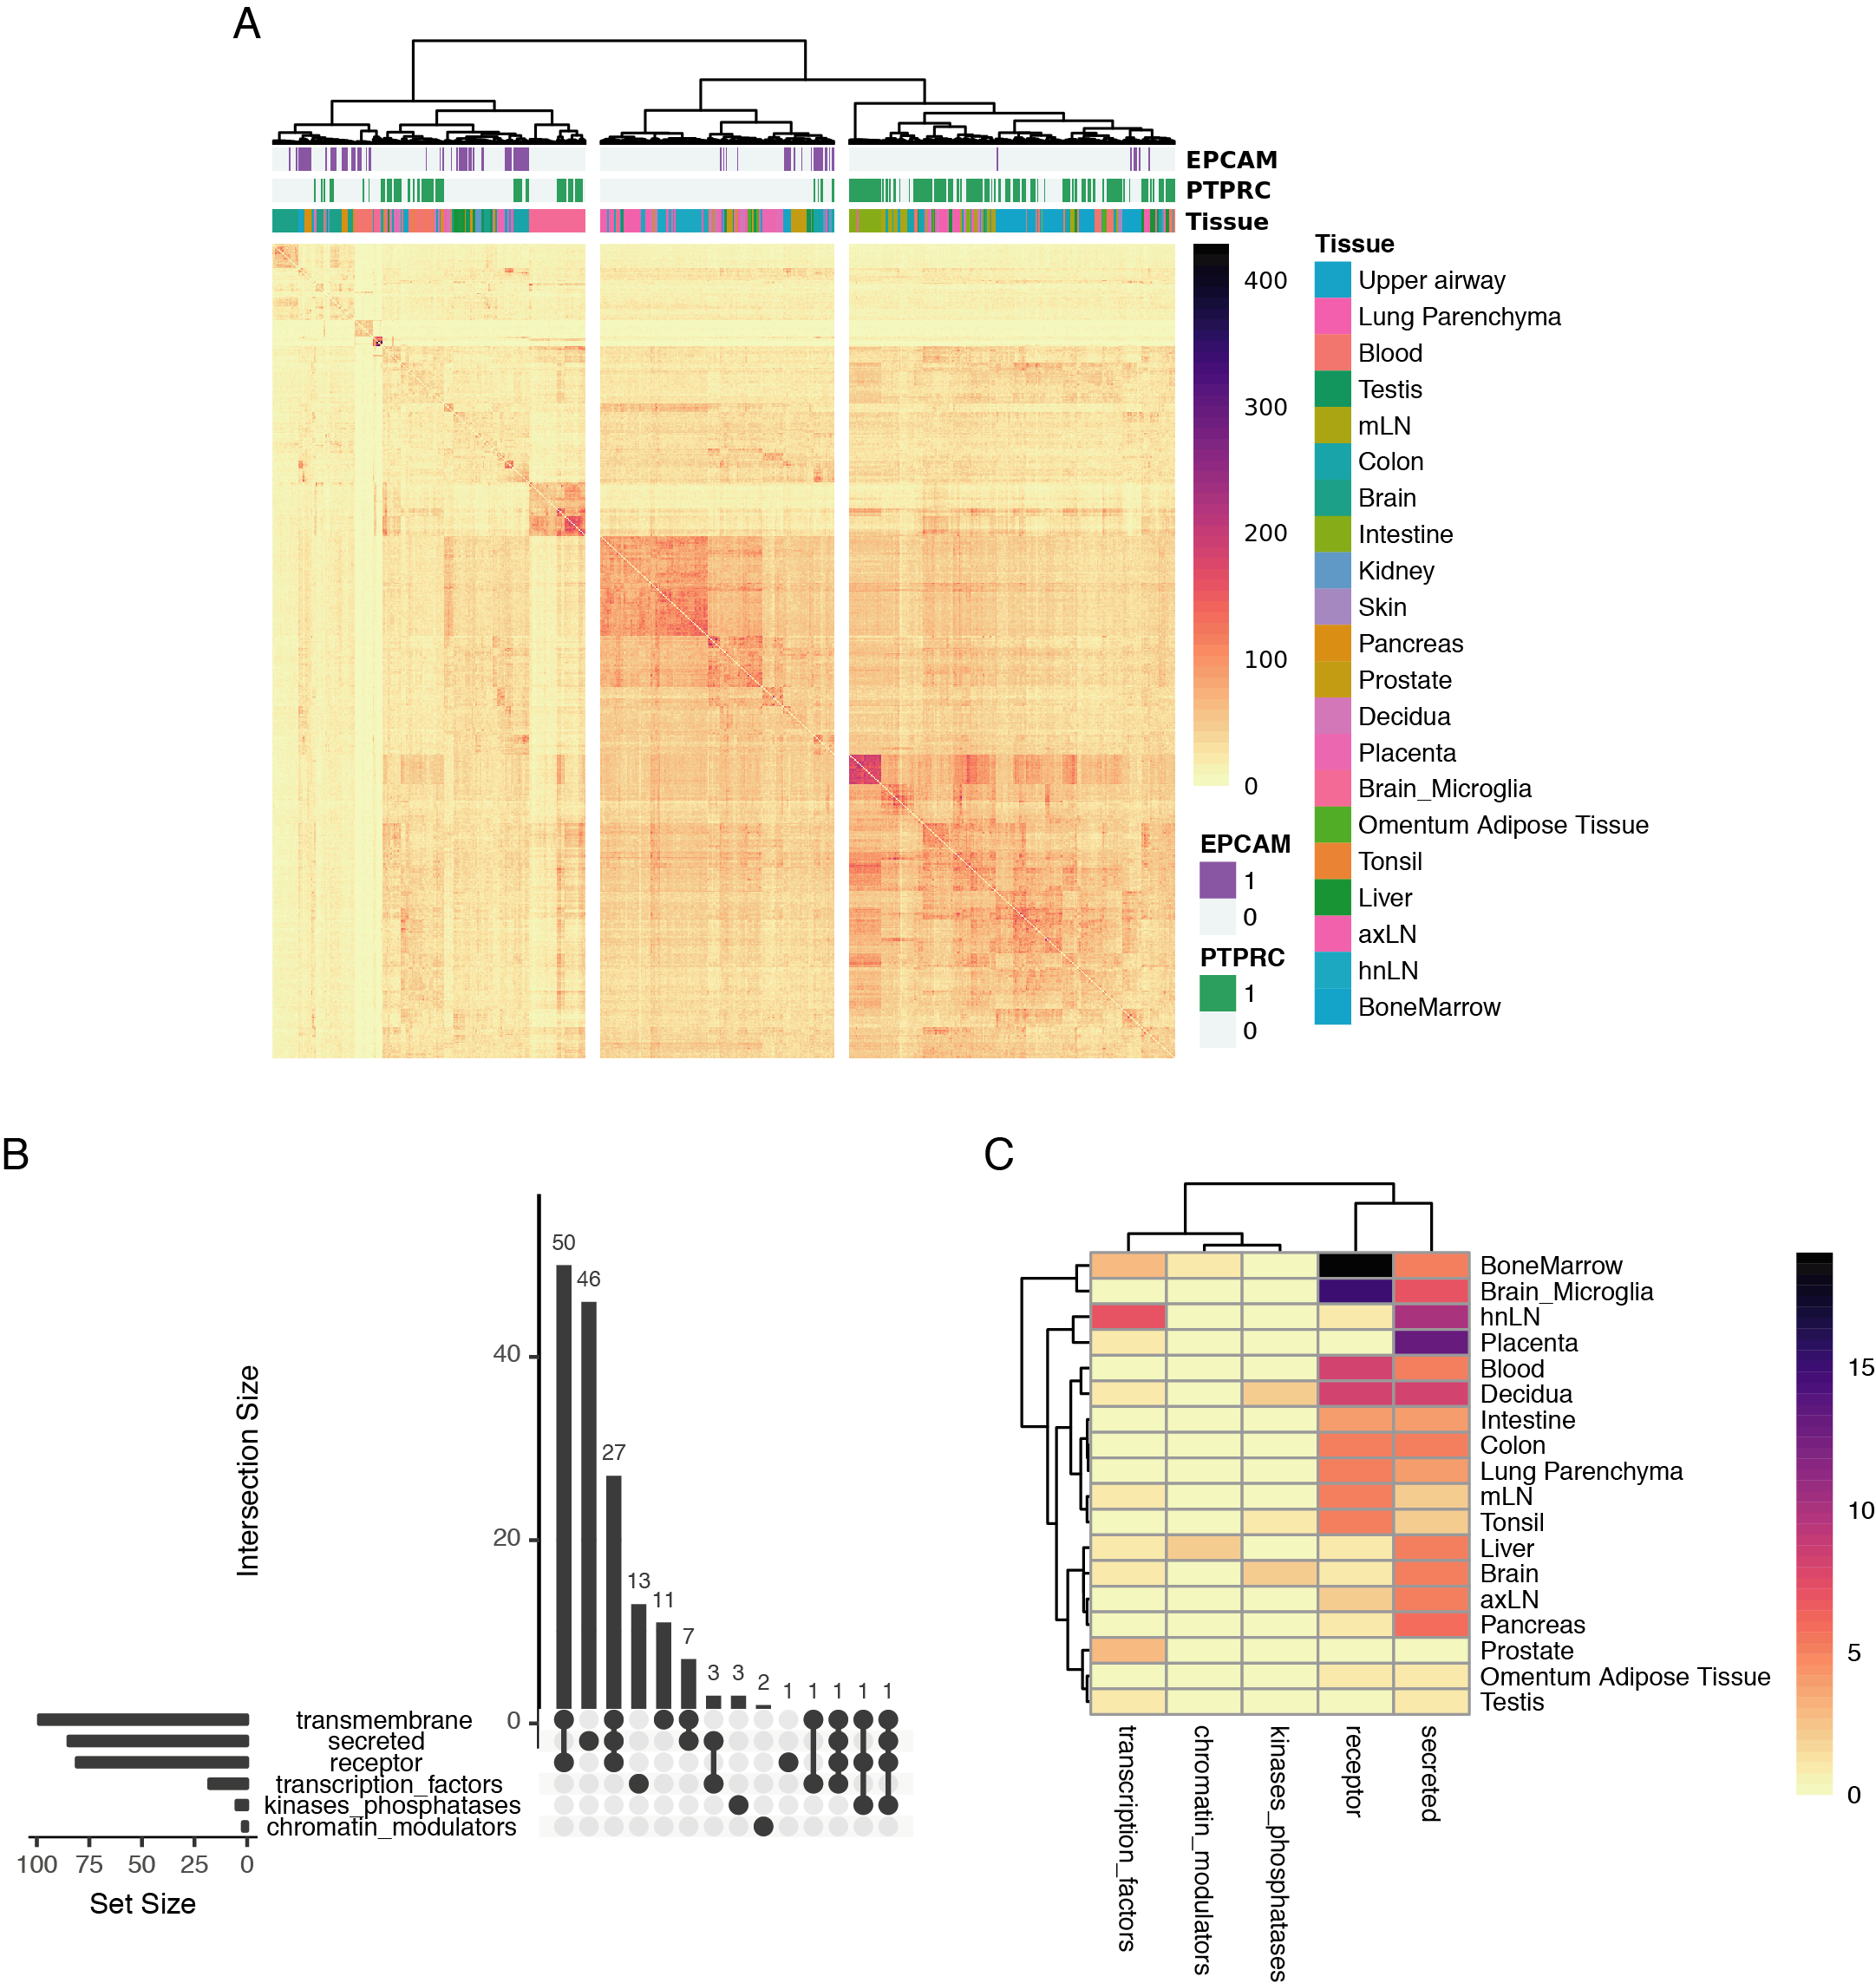
\includegraphics[width=1.0\textwidth]{Chapter4/Figs/chap4_genesAnalysis.png} % change word in curlies to change figure
    \caption[Genes driving cell identity definition across tissues]{\textbf{Genes driving cell identity definition across tissues}\newline\textbf{(A)} Clustered heatmap of the number of genes in common between pairs of \textit{CellTypist} clusters (thr1 = 0.99, thr2 = 0.8). Genes per cluster were determined as those with the top 500 coefficients as learned by the model. Values in the diagonal (number of genes per cluster, 500) were set to 0. \textbf{(B)} Upset plot counting the number of clusters enriched for a group of genes with a specific function. \textbf{(C)} Heatmap of number of clusters per tissue (y-axis) enriched for groups of genes with a specific function (x-axis).}
    \label{fig:chap4_genetypes}
\end{figure}

Relationships between clusters were probed by counting the number of pairwise shared genes. The top 500 genes were used to avoid a hard threshold across clusters, since the top coefficient values can be very variable between them. Clustering once more revealed a division between most immune and non-immune clusters (Figure~\ref{fig:chap4_genetypes}A). Moreover, various clusters containing cells from the same tissue were also grouped together, hinting at the existence of gene expression programmes shared by the different cell types within a tissue.

The concept of "cell type" is still inconclusively defined, yet it can be intimately related to a cell's molecular phenotype, i.e. the molecules driving cellular function. These drivers can either be the effector molecules directly responsible for the cell's array of functions, or the genomic regulators controlling the expression of genes involved in these functions. It has been showed that tissue-specificity at the gene expression level is mostly due to transcription factor-gene regulatory interactions~\citep{sonawane_understanding_2017}. The results from \textit{CellTypist} were used to assess what types of genes were more often at the top of the model coefficient rankings, which reflect the importance of expression of that gene in classifying a cell type. The following gene categories were tested for enrichment (see Methods Sections~\ref{section4.4_genelists} and~\ref{section4.4_enr}): Transcription Factors, Chromatin Modulators, Kinases and Phosphatases, Ligases and Deubiquitinases, Catalytic enzymes, Housekeeping genes, Receptors, Secreted proteins, Transmembrane proteins, and Peripheral membrane proteins. Analysis showed a consistent pattern for all surveyed models of predominantly enriched membrane and secreted proteins (Figure~\ref{fig:chap4_genetypes}B, Figure~\ref{fig:appB_supupset}). A number of clusters also had transcription factors enriched in their top hits, albeit in markedly lower number. Enrichment for the tested gene groups appeared evenly distributed across tissues, and did not group them in any meaningful manner (Figure~\ref{fig:chap4_genetypes}C). Lastly, it is also notable that only a fraction of the total clusters showed enrichment for any of the classes tested, which could be due to the restrictive test that only looks for enrichment at the very top genes, as well as the non-comprehensive list of functions tested.

These results point to the greater importance of the gene expression regulatory network's output molecules (genes coding for membrane and secreted proteins), in determining the identity of a cell.


\subsection{CellTypist as an operational reference for annotation}
\label{section_test}
% mention plans for a database
The operational goal of \textit{CellTypist} is to be used as an automatic classification framework for scRNA-seq data. Data integrated through the pipeline can be used as an unbiased model of cell identity to predict cell type labels in unannotated data.

\begin{figure}[pht!] 
\centering
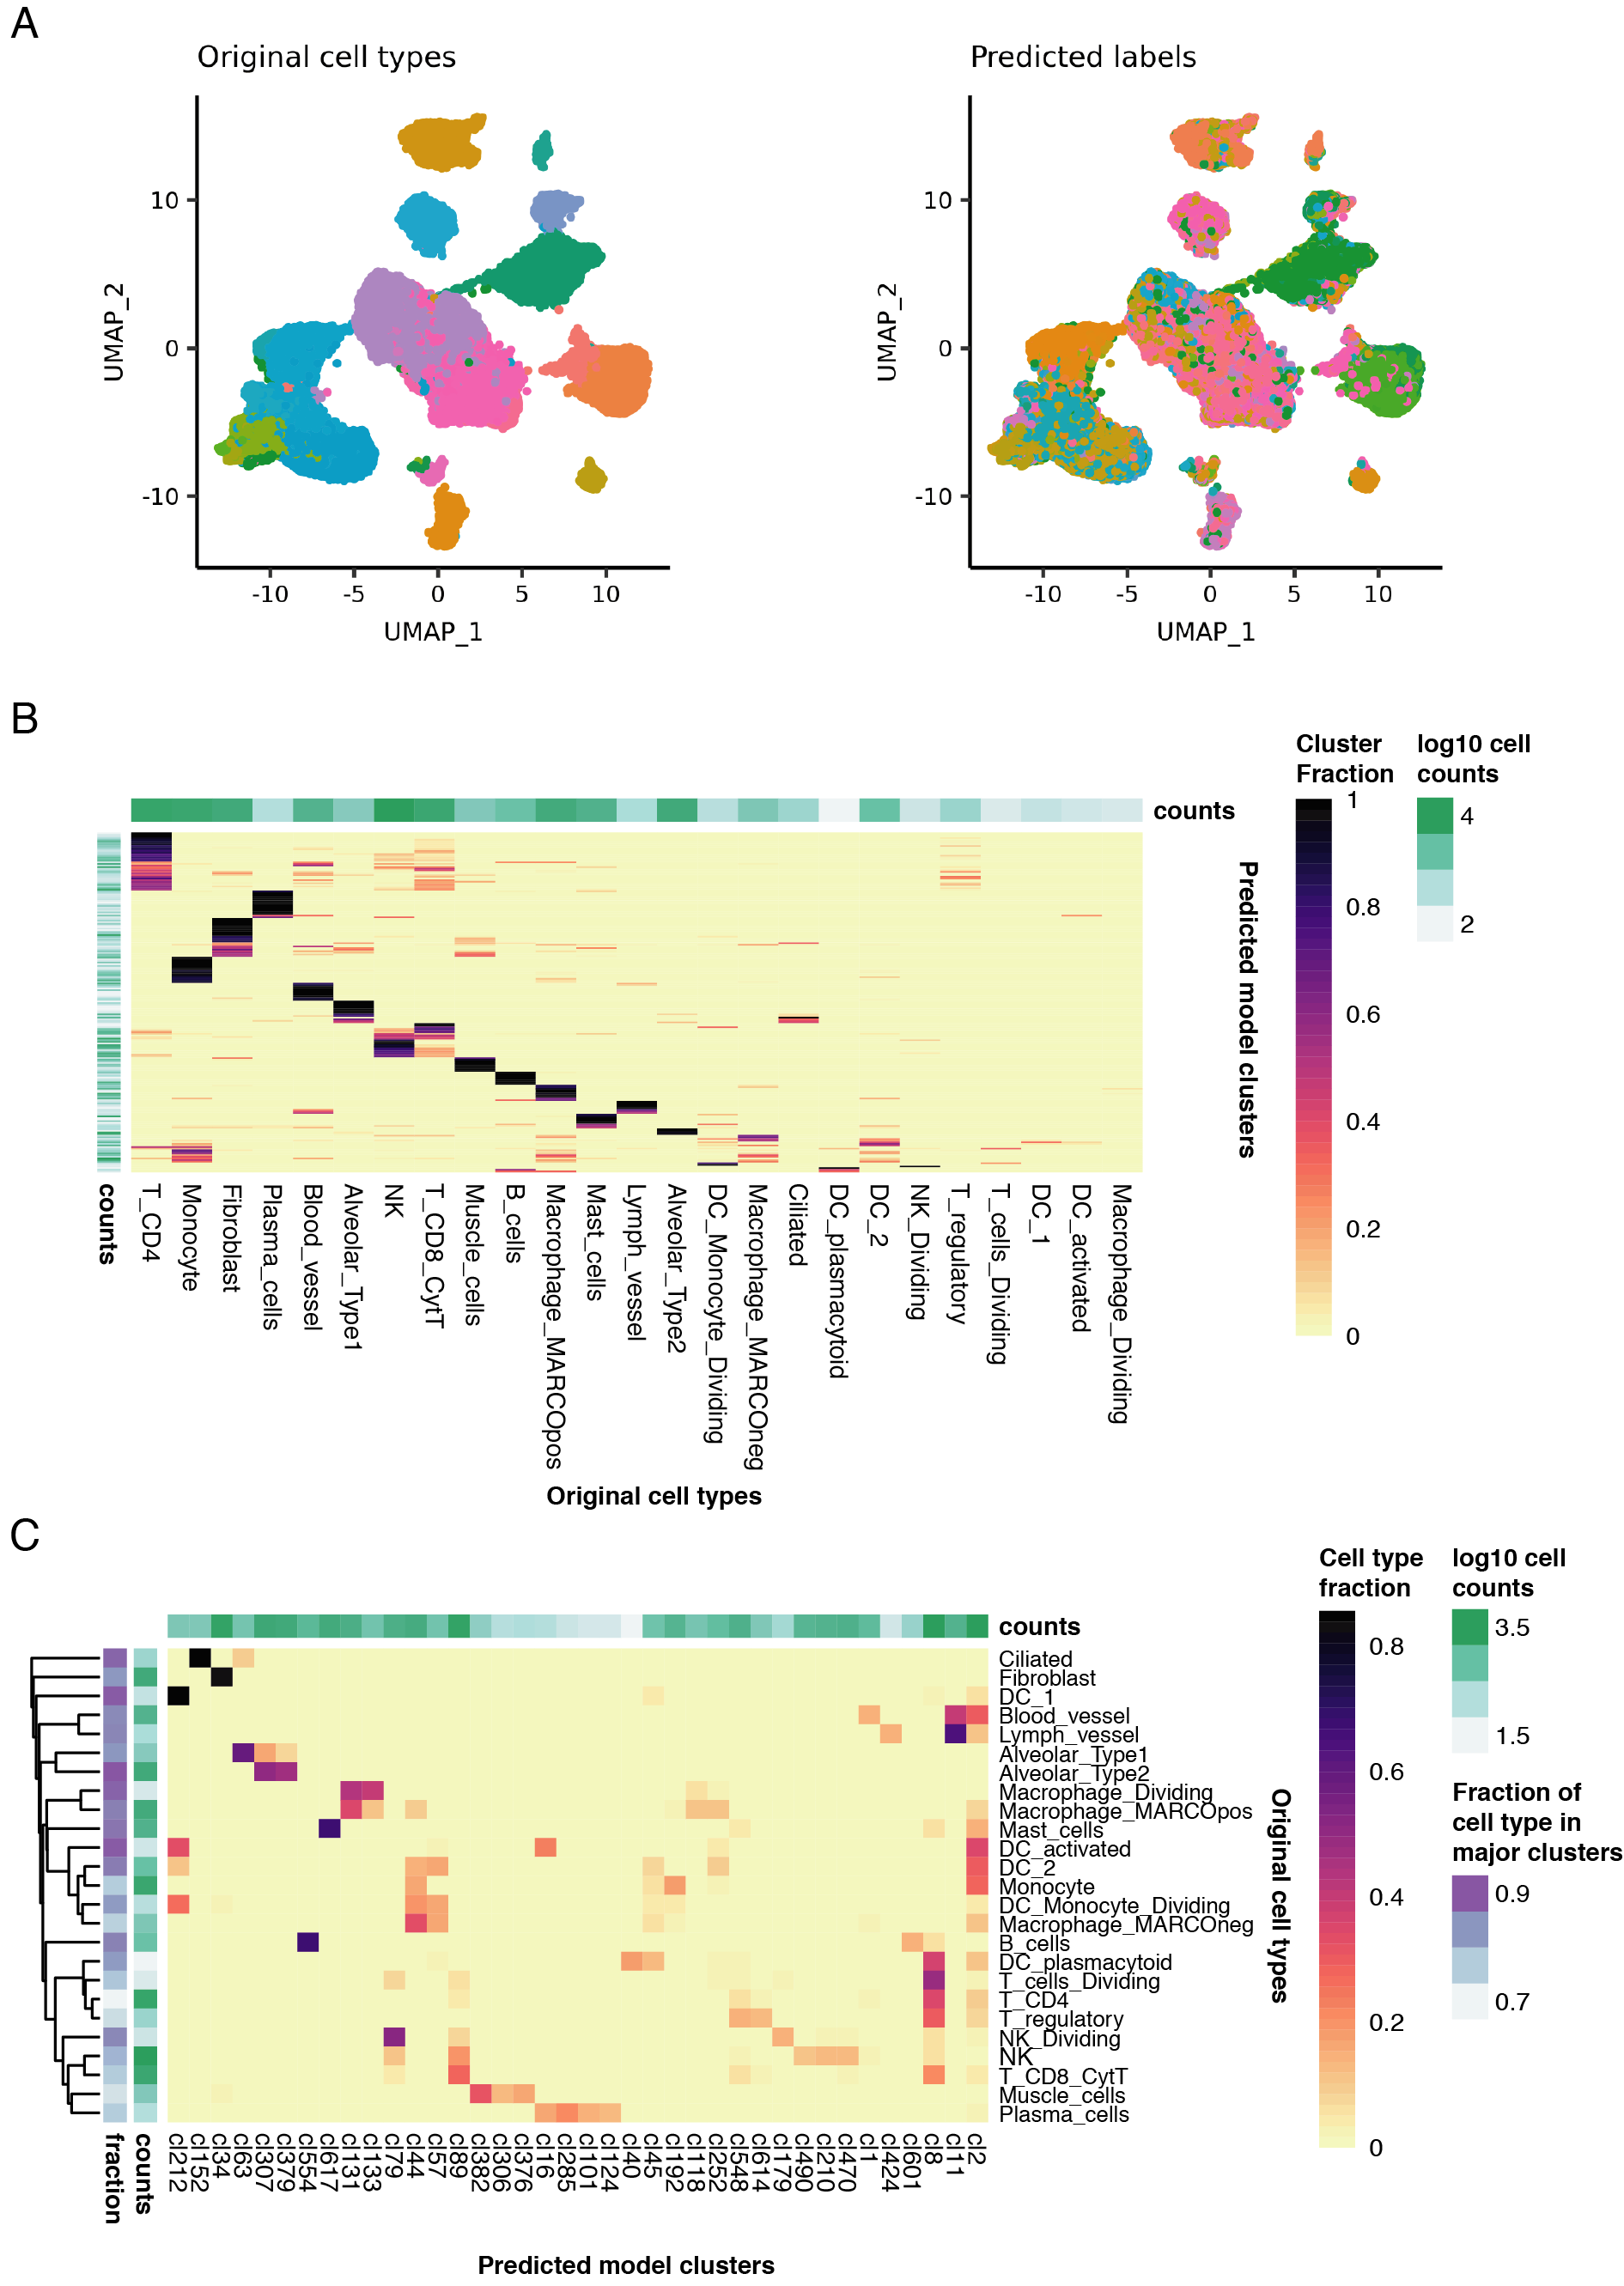
\includegraphics[scale=0.83]{Chapter4/Figs/chap4_preds.png} % change word in curlies to change figure
\caption[\textit{CellTypist} predictions for lung data from~\citep{madissoon_lung_2019}]{\textbf{\textit{CellTypist} predictions for lung data from~\citep{madissoon_lung_2019}}\newline\textbf{(A)} UMAP projections coloured by the original cell type annotations (left) and those predicted by \textit{CellTypist} (right) using thr1 = 0.99 and thr2 = 0.8. \textbf{(B)} Proportion of clusters (rows) matching each annotated cell type (columns). \textbf{(C)} Proportion of annotated cell types (rows) included in each cluster (columns). Only clusters including at least 10\% of a given cell type were included.}
\label{fig:chap4_preds}
\end{figure}

The data generated in~\citep{madissoon_lung_2019} was used to test the classification performance of \textit{CellTypist} with the compiled human data. This dataset was chosen because it includes three distinct tissues - lung, oesophagus, and spleen -, with only the first being represented in the collected datasets. More than 200.000 cells were collected from these three tissues, with various cell populations manually identified. The downside of this comparison is that the comparison can not be directly assessed, since the existing annotations for this dataset do not match those used by \textit{CellTypist}, which compiles a variety of nomenclatures used in each specific publication from where the data was obtained.

An overview of the classification results, projected in UMAP~\citep{mcinnes_umap:_2018} (Figure~\ref{fig:chap4_preds}A, Figure~\ref{fig:appB_oes}A, Figure~\ref{fig:appB_spleen}A), shows a similarity between the individual labelling of different clusters. The increased noise in \textit{CellTypist}'s annotations are likely due to the large number of categories it includes. Despite this, most model labels are highly specific, being attributed almost entirely to a single original cell type annotation (Figure~\ref{fig:chap4_preds}B, Figure~\ref{fig:appB_oes}B, Figure~\ref{fig:appB_spleen}B). While the opposite is not true (i.e. one cell type annotation can correspond to more than one cluster), it is nonetheless evident that each cell type is dominated by one or very few clusters (Figure~\ref{fig:chap4_preds}C, Figure~\ref{fig:appB_oes}C, Figure~\ref{fig:appB_spleen}C). Furthermore, even when excluding clusters including less than 10\% of cells from each annotated cell type (as is the case in the heatmap in Figure~\ref{fig:chap4_preds}C), the remaining clusters still include 70-90\% of cells (purple sidebar in Figure~\ref{fig:chap4_preds}C). A more careful look at the annotations present in the clusters that matched each original cell type in lung reveals the accuracy of the model. Type 2 alveolar cells matched clusters only containing that same annotation, whereas clusters in alveolar type 1 included type 1, and type 2, as well as secretory cells. Ciliated cells and fibrolasts mostly matched a single cluster each, in both cases composed of the exact same annotation. Cells annotated as "Lymph\_vessels" and "Blood\_vessels" both matched cl11 (containing "endothelium" and "lymphatic" cells), with the first also matching lymphatic endothelial cells from the axillary lymph node. T cell annotations were mostly assigned to cluster cl8, which includes a mix of CD4 and CD8 cells. In addition, T regulatory cells also matched cluster cl614, which includes activated T cells and Tregs. NK cells also matched a cluster with CD8 T cell annotation, but included two others containing mostly NK cells from other tissues. Lung cells that are derived from the myeloid lineage (Macrophages, Monocytes, Dendritic cells) all matched clusters mostly composed of these same annotations, albeit with some mix between them, which again demonstrates some of the difficulty that exists in separating these cell types.

% other models
The other models resulting from different parameters were also briefly examined. Despite the differences in number of clusters, all models show a similar specificity for the assigned clusters (Figure~\ref{fig:appB_othercl}). However, both models with fewer clusters (thr1 = 0.25, thr2 = 0.25; and thr1 = 0.1, thr2 = 0.1) both show less unique matching of original cell types to clusters (Figure~\ref{fig:appB_otherct}), with most of them matching the same larger clusters, which is likely an artifact of excessive merging within and across tissues (Figure~\ref{fig:chap3_combcl}A). 

Globally, it has been demonstrated that \textit{CellTypist} can be successfully used to annotate datasets with a broad diversity of cell types, and future improvements to the pipeline are likely to make it more precise in attributing cell identity. 


\section{Discussion}
\label{section4.3}
From its inception, the Human Cell Atlas (HCA) consortium has aimed to "define all human cell types in terms of distinctive molecular profiles (such as gene expression profiles)"~\citep{regev_human_2017}, a task that can not be easily accomplished by a single team. Beyond the financial and ethical constraints, collecting good quality scRNA-seq data requires tissue-specific knowledge, as well as profiling using both top-down and bottom-up approaches to obtain an overview of cell populations, while capturing cell type-specific phenotypic variations. Yet as data on human cells accumulates, methods capable of compiling the cellular census envisioned by the HCA members, and make it available to the community will be of great use.

% bias in collected data
%% model updating with new data will make it more inclusive/globally applicable
%% over represented cell types might "hide" smaller ones
%% data augmentation/downsampling can help
The human data here presented provides a broad overview of several organs. This leads the cell type reference generated by \textit{CellTypist} to be broadly applicable to new datasets. This reference is nonetheless also dependent of the way these tissues are sampled. Currently, many of them are mostly or totally composed of immune cell which, while adding valuable information about their diverse phenotypes, can also bias the model. Collecting more datasets is the ideal way of mitigating this problem, yet it can also be addressed by using data augmentiation or downsampling approaches~\citep{wong_understanding_2016,hie_geometric_2019}. This would be especially relevant at the model training step, as we have observed the clear impact of number of cells per label in classification accuracy (Figure~\ref{fig:chap3_model}C, Figure~\ref{fig:chap3_modelcl}C, Figure~\ref{fig:chap4_HA}D).

Consistent data integration is also essential to avoid redundant classes and misleading interpretations about cell type and tissue relationships. Data integration for scRNA-seq is still a heavily studied topic~\citep{haghverdi_batch_2018,lopez_deep_2018,polanski_bbknn:_2019, stuart_comprehensive_2019}, and can considerably influence the cell groupings detected in the data. \textit{CellTypist} is likely to evolve as a pipeline, in order to adopt a within- and cross-tissue integration framework that leads to a close reflection of the cell type information available for each dataset.

%tissue biology
Tissue identity relationships appear as an emergent result from the application of \textit{CellTypist}. The associations revealed between tissues are present at the cross-tissue integration stage (Figure~\ref{fig:chap4_tiss}A), and then also reflected in the top gens learned by the logistic regression model (Figure~\ref{fig:chap4_tiss}B). Furthermore, tissue identity is to some degree robust to incorrect or excessive grouping of single-cells (Figure~\ref{fig:appB_tissGSEA}), which reveals that tissues-specific expression programmes might be intrinsic to the core cell identity. The resolution of these tissue connections and programmes can be improved by broader cell type sampling and integration. This will allow the model to reveal a more fine-grained hierarchy beyond the immune/non-immune split, and ultimately map cellular phenotypes to a structured cell identity atlas.

% gene biology
%% more detailed conclusions can be taken once the reference is uniformly annotated/if more annotated data is included (because we can now go beyond tissues/clusters to actual cell types)
%% discuss how more accurate gene groups can give more accurate results
The data compiled offers for the first time a window into the drivers of cell identity. Analysis of enriched gene expression programmes can be improved by using a more uniform gene reference, as well as adopting more informative labels for the clusters obtained (which can come from improved dataset merging or manual annotation). Nonetheless, the analysis here showed consistently ranked receptors and secreted molecules above transcription factors when defining cell identity (Figure~\ref{fig:chap4_genetypes}B, Figure~\ref{fig:appB_supupset}). This is in agreement with previous reports~\citep{sonawane_understanding_2017}, yet this is the first instance where this type of analysis could achieve this level of cell type resolution. Importantly, defining which genes make up the core of cellular phenotypes is not the same as defining cell identity regulation. However, knowledge of the minimal gene expression set required to classify or obtain a determined phenotype (and consequently function) is a key point in understanding the operational definition of cell types. Thus, the expansion and improvement of the \textit{CellTypist} reference will increasingly provide a foundation to understanding how cell types arise and evolve~\citep{zimmermann_ancient_2019}, and will help prioritise gene targets for effective cellular engineering.

% use and availability of this data collection
This large human cell type reference can be very useful to characterise cell identity in a variety of systems. In disease-focused studies, the steady-state reference provided by \textit{CellTypist} can automatically annotate the cells obtained from a disease sample, eliminating the need to obtain a matching healthy sample. Another potential use is to characterise cell fates and heterogeneity when differentiating organoids. Classifying scRNA-seq data from the generated organoids using an unbiased reference can reveal the cell types present that a specific protocol was able to differentiate. \textit{CellTypist} will also be available as an online resource, where the model can be directly used, and is accompanied by a database showing the defining characteristics of each cell type - marker genes detected, tissues of origin, datasets characterising them, and similar cell types. This is further intended to be articulated with a Cell Ontology~\citep{bard_ontology_2005}, and have cell names be consistently used when new data is produced, with a direct correspondence to both databases. Lastly, future releases of \textit{CellTypist} models will include more species, adding an evolutionary layer to our knowledge of cell identity.


\section{Methods}
\label{section4.4}
\subsection{Collecting single-cell expression data}
\label{section4.4_datacol}
Single-cell RNA-seq expression data was collected for the publications listed in Table~\ref{table:tab_4_1}, together with cell type annotations when there were available. Information about tissue, donor type and scRNA-seq protocol were obtained from the publications.

In most cases, count data was available together with the raw sequencing reads in the chosen repository. In other cases, the expression matrices deposited included log normalised data. This means that the data was normalised by the total number of reads/UMI of each cell, often followed by multiplication by a specific scaling factor (usually 10000), and finally log scaled, adding 1 to account for the zeroes present. For these datasets, data was reconverted to counts following an approach similar to that explained in \url{http://www.nxn.se/valent/2018/10/25/unscaling-scaled-counts-in-scrna-seq-data}. Briefly, given the scaling factor \textit{S}, representing the second most abundant value for each cell, and \textit{x} for each expression value, unscaled data \textit{U} was obtained by applying Formula 4.1, followed by rounding to the nearest unit to remove floating point inaccuracies.

\begin{align}
U = \frac{\mathrm{e}^{x} - 1}{S}
\end{align}

Raw count matrices were then compiled together, guaranteeing as much correspondence as possible between the diverse gene references used. All gene identifiers were mapped to the corresponding HGNC gene names, and all unique identifiers were kept.


\subsection{\textit{CellTypist} parameter optimisation and training}
\label{section4.4_model}
The \textit{CellTypist} pipeline was applied to the complete human dataset. Data from the same tissues was integrated and clustered using the Leiden algorithm~\citep{traag_louvain_2019} at several resolutions. For tissues with cell type annotations, resolution was optimised using the split-join distance~\citep{dongen_performance_2000} between clusters and cell type annotation and constrained to a number of clusters at least as large as the number of cell type annotations in the largest collected dataset (Figure~\ref{fig:chap4_HA}A, see also Chapter~\ref{chap:CT_method} Section~\ref{section3.2.1}).

Following clustering, per tissue logistic regression models were trained, running for 10 epochs of a maximum of 100 iterations each. These models were used to run the cross-tissue cluster merging pipeline (Chapter~\ref{chap:CT_method} Section~\ref{section3.2.2}), and a combination of parameters was chosen based on the ratio of split-join distances (merged vs annotated cell types over per tissue vs annotated cell types) (Figure~\ref{fig:chap4_HA}B), resulting in the choice of thr1 = 0.99 and thr2 = 0.8. Additionally, three other combinations were chosen for comparison: thr1 = 0.4 and thr2 = 0.99, the combination with the top split-join ratio when only considering merged clusters (Figure~\ref{fig:appB_grids}C, Figure~\ref{fig:appB_moremodels}A-B); thr1 = 0.25 and thr2 = 0.25, one of the combinations with the highest fraction of merged clusters (Figure~\ref{fig:appB_grids}B, Figure~\ref{fig:appB_moremodels}C-D); thr1 = 0.1 and thr2 = 0.1, the combination with the highest fraction of merged clusters, as well as highest split-join fraction (Figure~\ref{fig:appB_grids}B, Figure~\ref{fig:appB_moremodels}E-F).

The groupings obtained were used to train a logistic regression model (Chapter~\ref{chap:CT_method} Section~\ref{section3.2.3}) that run for 25 epochs of a maximum of 100 iterations each, using 90\% of the data as a training set, and the remaining as a left out test set that was tested at every iteration (Figure~\ref{fig:chap4_HA}C-D, Figure~\ref{fig:appB_moremodels}).


\subsection{Obtaining gene group lists}
\label{section4.4_genelists}
The groups of genes here presented were chosen to reflect various broad functions present in cells. They are not exhaustive, and overlaps between gene sets exist due to the ambiguity of some categories.

\textit{GO Terms}: GO Terms were downloaded using the biomaRt R package~\citep{durinck_mapping_2009}. Genes from different terms were then grouped in the following categories (similar to~\citep{hagai_gene_2018}): chromatin modulators (GO:0006338 (chromatin remodelling), GO:0003682 (chromatin binding), GO:0042393 (histone binding), and GO:0016568 (chromatin modification)); kinases and phosphatases (GO:0004672 (protein kinase activity) and GO:0004721 (phosphoprotein phosphatase activity)) and catalytic enzymes (GO:0003824 (catalytic activity)).

\textit{Transcription Factors}: Human transcription factors were obtained from AnimalTFDB v3.0 (~\url{http://bioinfo.life.hust.edu.cn/AnimalTFDB/})~\citep{hu_animaltfdb_2019}.

\textit{Housekeeping genes}: Housekeeping genes were obtained from~\url{https://m.tau.ac.il/~elieis/HKG/}~\citep{eisenberg_human_2013}.

\textit{Cell communication-associated genes}: Genes involved in cell-cell communication were obtained from~\url{cellphonedb.org}~\citep{efremova_cellphonedb_2019}. Only genes annotated as "transmembranar", "secreted", "peripheral", and "receptor" were kept. Given the structure of the annotation in this database, some genes are included in more than one group. In particular, most receptors and some secreted proteins are also classified as transmembranar.

\textit{Tissue-specific genes}: Tissue specific genes were determined as described in~\citep{sonawane_understanding_2017}. Briefly, RNA-seq expression data from the GTex Consortium was obtained (~\url{https://gtexportal.org/home/index.html})~\citep{consortium_genotype-tissue_2015}, and genes were considered tissue-specific for a given tissue if the difference between their median expression in that tissue and across all tissues normalised by its inter quartile range across all tissues, was greater than 2.


\subsection{Enrichment of gene groups}
\label{section4.4_enr}
To obtain enriched groups of genes (Sections~\ref{section_tissues} and~\ref{section_genes}), the top 500 genes based on their model coefficients were obtained for each cluster. Gene Set Enrichment Analysis (GSEA)~\citep{subramanian_gene_2005} was performed using the liger R package (\url{https://cran.rstudio.com/web/packages/liger/index.html}), considering the gene sets as defined in Section~\ref{section4.4_genelists}. Enrichment was deemed signifficant if the q-value was lower than 0.05, and if the enrichment score was positive, signifying an enrichment in the top genes. In heatmaps plotting GSEA results (Figure~\ref{fig:chap4_tiss}B-D; Figure~\ref{fig:appB_tissGSEA}), the colour scale is capped at 0.8 (fraction of enriched clusters per tissue), and the annotation scales are capped at 0.5 (fraction of clusters with mean expression of the indicated gene of at least 1). Clusters merge across tissues were only counted towards the tissue contributing the most cells to them.


